\section{Auswertung}
\label{sec:Auswertung}
\subsection{Bestimmung der Winkelrichtgröße}

Durch Aufstellung der Drehmomentsgleichung der Drillachse und dem Umstellen nach der Winkelrichtgröße folgt
\begin{equation}
	D = \frac{ |F| \cdot |r|}{\varphi} \ .
\end{equation}
Für die verwendete Torsionsfeder folgt, für die gemessenen Kräfte und einem Radius von
\begin{align*}
	r = (\num{90.7 +- 0.4}) \, \text{mm}
\end{align*}
Winkelrichtgrößen von

\begin{table}[ht]
	\centering
	\caption{Winkelrichtgrößen für die einzelen gemessenen Daten}
	\label{tab:winkelrichtgröße}
	\begin{tabular}{c c c c}
		\toprule
		$\varphi$ / Grad & $\varphi$ / rad & $F$ / $10^{-1}$ N & $D$ / $10^{-2}$ Nm \\
		\midrule
		15 & 0.26 & 0.6 & \num{2.1 +- 1.4} \\
		30 & 0.52 & 1.2 & \num{2.1 +- 0.7} \\
		45 & 0.79 & 1.5 & \num{1.7 +- 0.4} \\
		50 & 0.87 & 2.2 & \num{2.3 +- 0.5} \\
		60 & 1.05 & 2.8 & \num{2.4 +- 0.5} \\
		75 & 1.31 & 3.4 & \num{2.4 +- 0.3} \\
		90 & 1.57 & 3.7 & \num{2.1 +- 0.3} \\
		105& 1.83 & 4.4 & \num{2.2 +- 0.2} \\
		120& 2.10 & 5.1 & \num{2.2 +- 0.2} \\
		135& 2.36 & 5.6 & \num{2.2 +- 0.2} \\
		\bottomrule
	\end{tabular}
\end{table}

Die Messunsicherheit berechnet sich aus einem Ablesefehler des Winkels von $\le 3^\circ $ und der Kraft von $\le 0.02$ N. Nach Mittelung der Werte und Fehlerfortpflanzung (siehe Formel \ref{eqn:Gauß}) erhält man eine Winkelrichtgröße von
\begin{align*}
	D_\text{0} = (\num{2.16 +- 0.19}) \cdot 10^{-2} \, \text{Nm} \ .
\end{align*}


\subsection{Bestimmung des Eigenträgheitsmoments}
Um das Trägheitsmoment der Drillachse $I_\text{D}$ zu berechnen muss zuerst einmal das Trägheitsmoment des nahezu masselosen Stabes $I_\text{S}$ bestimmt werden. Zusätzlich muss das Trägheitsmoment der beiden am Stab befestigten Gewichte $2 \cdot I_\text{G}$ berechnet werden. Das Trägheitsmoment des Stabes beträgt in dem gewählten Versuchsaufbau bei einer Masse von
\begin{align*}
	m = 96,26 \, \text{g}
\end{align*}
und einer Länge von
\begin{align*}
	l = 60 \, \text{cm}
\end{align*}
\begin{equation}
	I_\text{S} = \frac{ml^2}{12}= 2.85 \cdot 10^{-3} \, \text{kg m} \ .
\end{equation}
Für die vom Schwerpunkt um die Strecke $a$ verschobenen Zylinder ergibt sich nach Formel \ref{eqn:Steiner} ein Trägheitsmoment $I_\text{G}$ von (siehe Tabelle \ref{tab:I_D})
\begin{equation}
	I_\text{G}= I_\text{Schwerpunkt}+ I_\text{Steiner} = m (\frac{R^2}{4} + \frac{h^2}{12}) + m \cdot a^{2}
\end{equation}
Mit Hilfe einer linearen Regression soll das Trägheitsmoment der Drillachse bestimmt werden. Dafür wird Formel \ref{eqn:Schwingungsdauer} quadriert und das Trägheitsmoment
\begin{align*}
	I_\text{ges} = I_\text{D} + 2 \cdot I_\text{G}
\end{align*}
in die Formel eingesetzt.
\begin{table}[ht]
        \centering
        \caption{Abstände der Gewichte von der Drehachse und fünfache Periodendauer}
        \label{tab:I_D}
        \begin{tabular}{c c}
                \toprule
                $a$ / mm & $T$ / s  \\
                \midrule
                40 & 2.53  \\
                65 & 2.95  \\
                90 & 3.50  \\
                115& 3.99  \\
                140& 4.59  \\
                165& 5.22  \\
                190& 5.90  \\
                215& 6.55  \\
                240& 7.11  \\
                265& 7.85  \\

                \bottomrule
        \end{tabular}
\end{table}
Um einen Koeffizientenvergleich zwischen der Regression und der quadratischen Schwingungsdauer zu machen, werden die Therme wie folgt sortiert.
\begin{equation}
	\underbrace{T^2}_y = \underbrace{\frac{8 \pi^2 m_\text{G}}{D}}_m \underbrace{a^2}_x + \underbrace{\frac{4 \pi^2 I_\text{D}}{D} + \frac{8\pi^2 m_\text{G}}{D} \left( \frac{R^2}{4} + \frac{h^2}{12} \right)}_b
\end{equation}
Die Steigung $m$ berechnet sich nach Formel \ref{eqn:m} und der Koeffizeientvergleich ergibt
\begin{align}
	m = \num{798 +- 6} = \frac{8 \pi^2 m_\text{G}}{D}
\end{align}
Daraus ergibt sich eine Winkelrichtgröße von
\begin{align}
	D = (\num{2.16 +- 0.02}) \cdot 10^{-2} \, \text{Nm} \ .
\end{align}
Das Trägheitsmoment der Drillachse errechnet sich aus dem vergleich zwischen dem errechnetem Wert der Regression und der gemessenen Werte.
\begin{align}
	b = \frac{4 \pi^2 I_\text{D}}{D} + \frac{8\pi^2 m_\text{G}}{D} \left( \frac{R^2}{4} + \frac{h^2}{12} \right) = 5.48
\end{align}
Nach Umstellen der Formel nach $I_\text{D}$, beträgt das Trägheitsmoment der Drillachse
\begin{align*}
	I_\text{D} = (\num{2.8 +- 1.9}) \cdot 10^{-3} \, \text{kg m}^2 \ .
\end{align*}




\subsection{Trägheitsmomente verschiedener Objekte}
\subsubsection{Kugel}
Durch Mittelung und Gauß'scher Fehlerfortpfortpflanzung (siehe Kapitel \ref{sec:Fehler}) erhält man einen Wert für den Durchmesser von
\begin{equation}
	d = (\num{137.44 +- 0.022}) \, \text{mm} \ .
\end{equation}
Das Trägheitsmoment einer Kugel berechnet sich aus
\begin{align}
	I_\text{K,theo} = \frac{2}{5} mr^2 \ .
\end{align}
Bei einer Masse von
\begin{align*}
	m = 0.8126 \, \text{kg}
\end{align*}
beträgt das theoretische Trägheitsmoment der Kugel
\begin{align}
	I_\text{K,theo} = 1.53 \, \text{kg m}^2 \ .
\end{align}
Das experimentell ermittelte Trägheitsmoment errechnet sich durch Umformung der Formel \ref{eqn:Schwingungsdauer} und ergibt nach Mittelung der Periodendauer
\begin{equation}
	\label{eqn:T_K}
	I_\text{K,exp} = \left( \frac{T}{2 \pi} \right) ^2 \cdot D = (\num{1.62 +- 0.14}) \cdot 10^{-3} \, \text{kg m}^2
\end{equation}

\subsubsection{Zylinder}
Das theoretische Trägheitsmoment des Zylinders wird aus
\begin{align}
	I_\text{Z,theo} = \frac{1}{2} mr^2
\end{align}
berechnet. Durch Einsetzen des Radius von
\begin{align*}
	r = (\num{4.0 +- 0.0}) \cdot 10^{-2} \, \text{m}
\end{align*}
ergibt sich ein Trägheitsmoment von
\begin{align}
	I_\text{Z,theo} = 1.58 \cdot 10^{-3} \, \text{kg m}^2 \ .
\end{align}
Das experimentelle Trägheitsmoment berechnet sich analog zur Kugel (siehe Formel \ref{eqn:T_K}) und beträgt
\begin{align}
	I_\text{Z,exp} = (\num{1.54 +- 0.13}) \cdot 10^{-3} \, \text{kg m}^2 \ .
\end{align}

\subsection{Trägheitsmoment der Puppe}
Durch Einteilen der Puppe in verschieden große Zylinder soll das Trägheitsmoment der Puppe bestimmt werden. Dafür werden mehrere Maße der einzelnen Zylinder genommen um einen möglichst genauen Mittelwert zu erlangen. Die Maße, Massen und Trägheitsmomente der Zylinder sind der Tabelle zu entnehmen.
\begin{table}
	\centering
	\caption{Maße, Gewicht und Trägheitsmomente der Körperteile}
	\label{tab:Puppe}
	\begin{tabular}{l c c c c}
		\toprule
		$  $ & $Kopf$ & $Rumpf$ & $Bein$ & $Arm$ \\
		\midrule
		Durchmesser 	$10^{-3}$ \, m	& \num{24.5 +- 7.1}	&\num{35.0 +- 5.8}      &\num{15.5 +- 2.8}	&\num{13.1 +- 3.1}	\\
		Höhe 		$10^{-3}$ \, m	& \num{56.0 +- 0.5}	&\num{97.2 +- 2.5}      &\num{150.0 +- 4.0}	&\num{139.6 +- 0.8}	\\
		Volumen		$10^{-5}$ \, m$^3$& \num{2.2 +- 1.3}	&\num{9.4 +-3.1}	&\num{2.8 +- 1}		&\num{1.9 +- 0.9}	\\
		Masse		$10^{-2}$ \, kg	& \num{2.0 +- 1.2}      &\num{7.1 +- 2.8}       &\num{2.1 +- 0.9}       &\num{1.4 +- 0.7}       \\
		Trägheitsmoment			&	&	&	&	\\
		angelegt	$10^{-6}$ \, kg \cdot m$^2$	& \num{1.5 +- 1.3}     	&\num{10.9 +- 5.6}       &\num{1.9 +- 1.0}       &\num{5.3 +- 3.1}      \\
		ausgestreckt	$10^{-6}$ \, kg \cdot m$^2$	& \num{1.5 +- 1.3}    	&\num{10.9 +- 5.6}       &\num{1.9 +- 1.0}       &\num{110 +- 60}       \\
		\bottomrule
	\end{tabular}
\end{table}
Dabei wird angenommen, dass die Puppe eine homogene Dichte und die Masse besitzt. Aus der Beziehung
\begin{align}
	M = \varrho \cdot V = 162.7 \, \text{g}
\end{align}
lassen sich die Massen der unterschiedlichen Zylinder bestimmen. Die einzelnen Trägheitsmomente setzen sich jeweils aus den Schwerpunktsträgheitsmomenten der Zylinder zusammen und dem Steiner Anteil. Daraus ergeben sich nach Summe der einzelnen Trägheitsmomente aus Tabelle \ref{tab:Puppe} ein Gesamtträgheitsmoment für die Puppe mit angelegten Armen von
\begin{align}
	I_\text{an} = (\num{2.7 +- 1.0}) \cdot 10^{-5} \, \text{kg m}^2
\end{align}
und für die Puppe mit ausgestreckten Armen von
\begin{align}
	I_\text{aus} = (\num{2.5 +- 1.2}) \cdot 10^{-4} \, \text{kg m}^2 \ .
\end{align}
\ \\
Die praktische Bestimmung des Trägheitsmoments der Puppe erfolgt durch die Messung der Schwingungsdauer.
\begin{table}
	\centering
	\label{tab:TP}
	\caption{Fünfache Periodendauer der Puppe}
	\begin{tabular}{c c}
		\toprule
		$t_\text{an}$ / s & $t_\text{aus}$ / s \\
		\midrule
		2.80&3.84\\
		3.00&3.64\\
		3.01&3.87\\
		2.90&3.83\\
		2.87&3.84\\
		\bottomrule
	\end{tabular}
\end{table}
Durch Anwendung der Formel \ref{eqn:T_K} ergibt sich ein Trägheitsmoment $I_\text{aus}$ für die gesamte Puppe mit ausgestreckten Armen von
\begin{equation}
	I_\text{aus} = (\num{3.17 +- 0.30}) \cdot 10^{-4} \, \text{kg m}^2
\end{equation}
Die Berechnung des Trägheitsmomentes mit angelegten Armen folgt analog und beträgt
\begin{align}
	I_\text{an} = (\num{1.86 +- 0.19}) \cdot 10^{-4} \, \text{kg m}^2 \ .
\end{align}

%\begin{figure}
%  \centering
%  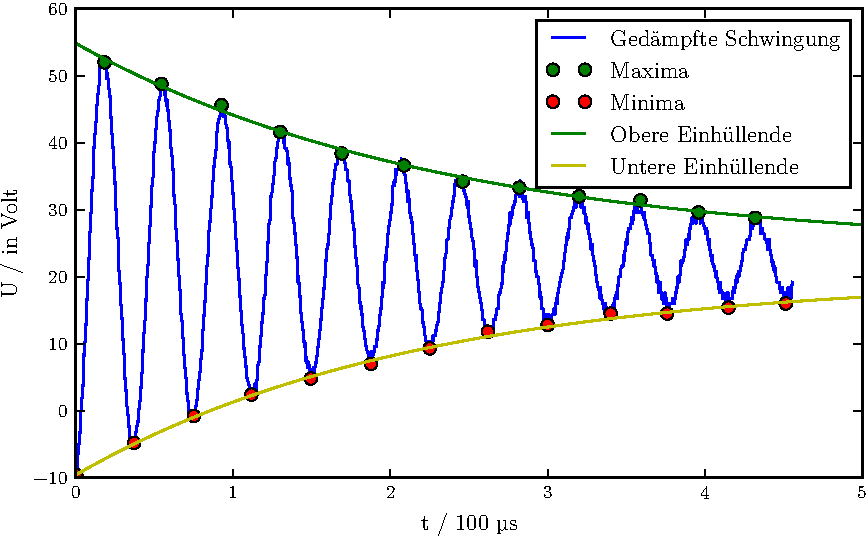
\includegraphics{plot.pdf}
%  \caption{Plot.}
%  \label{fig:plot}
%\end{figu
